%-*- ES -*-
%----------------------------------------------------------------------
% Capitulo 7: Descripción del problema

En éste capítulo se verá por qué los protocolos http y smtp son inseguros, introducción al snnifin, spoofing, arp attack
%----------------------------------------------------------------------

(Agregar una intro)

\section{Establishing Authority}

HTTP relies on the notion of an authoritative response: a response
that has been determined by (or at the direction of) the authority
identified within the target URI to be the most appropriate response
for that request given the state of the target resource at the time
of response message origination.  Providing a response from a
non-authoritative source, such as a shared cache, is often useful to
improve performance and availability, but only to the extent that the
source can be trusted or the distrusted response can be safely used.

Unfortunately, establishing authority can be difficult.  For example,
phishing is an attack on the user's perception of authority, where
that perception can be misled by presenting similar branding in
hypertext, possibly aided by userinfo obfuscating the authority
component (see Section 2.7.1).  User agents can reduce the impact of
phishing attacks by enabling users to easily inspect a target URI
prior to making an action, by prominently distinguishing (or
rejecting) userinfo when present, and by not sending stored
credentials and cookies when the referring document is from an
unknown or untrusted source.

When a registered name is used in the authority component, the "http"
URI scheme (Section 2.7.1) relies on the user's local name resolution
service to determine where it can find authoritative responses.  This
means that any attack on a user's network host table, cached names,
or name resolution libraries becomes an avenue for attack on
establishing authority.  Likewise, the user's choice of server for
Domain Name Service (DNS), and the hierarchy of servers from which it
obtains resolution results, could impact the authenticity of address
mappings; DNS Security Extensions are one way to
improve authenticity.

Furthermore, after an IP address is obtained, establishing authority
for an "http" URI is vulnerable to attacks on Internet Protocol
routing.


\section{Risks of Intermediaries}

By their very nature, HTTP intermediaries are men-in-the-middle and,
thus, represent an opportunity for man-in-the-middle attacks.
Compromise of the systems on which the intermediaries run can result
in serious security and privacy problems.  Intermediaries might have
access to security-related information, personal information about
individual users and organizations, and proprietary information
belonging to users and content providers.  A compromised
intermediary, or an intermediary implemented or configured without
regard to security and privacy considerations, might be used in the
commission of a wide range of potential attacks.

Intermediaries that contain a shared cache are especially vulnerable
to cache poisoning attacks.
Implementers need to consider the privacy and security implications
of their design and coding decisions, and of the configuration
options they provide to operators (especially the default
configuration).

Users need to be aware that intermediaries are no more trustworthy
than the people who run them; HTTP itself cannot solve this problem.

\section{Attacks via Protocol Element Length}

Because HTTP uses mostly textual, character-delimited fields, parsers
are often vulnerable to attacks based on sending very long (or very
slow) streams of data, particularly where an implementation is
expecting a protocol element with no predefined length.



\section{Response Splitting}

Response splitting (a.k.a, CRLF injection) is a common technique,
used in various attacks on Web usage, that exploits the line-based
nature of HTTP message framing and the ordered association of
requests to responses on persistent connections [Klein].  This
technique can be particularly damaging when the requests pass through
a shared cache.

Response splitting exploits a vulnerability in servers (usually
within an application server) where an attacker can send encoded data
within some parameter of the request that is later decoded and echoed
within any of the response header fields of the response.  If the
decoded data is crafted to look like the response has ended and a
subsequent response has begun, the response has been split and the
content within the apparent second response is controlled by the
attacker.  The attacker can then make any other request on the same
persistent connection and trick the recipients (including
intermediaries) into believing that the second half of the split is
an authoritative answer to the second request.

For example, a parameter within the request-target might be read by
an application server and reused within a redirect, resulting in the
same parameter being echoed in the Location header field of the
response.  If the parameter is decoded by the application and not
properly encoded when placed in the response field, the attacker can
send encoded CRLF octets and other content that will make the
application's single response look like two or more responses.


\section{Request Smuggling}

Request smuggling ([Linhart]) is a technique that exploits
differences in protocol parsing among various recipients to hide
additional requests (which might otherwise be blocked or disabled by
policy) within an apparently harmless request.  Like response
splitting, request smuggling can lead to a variety of attacks on HTTP
usage.


\section{Message Integrity}

HTTP does not define a specific mechanism for ensuring message
integrity, instead relying on the error-detection ability of
underlying transport protocols and the use of length or
chunk-delimited framing to detect completeness.  Additional integrity
mechanisms, such as hash functions or digital signatures applied to
the content, can be selectively added to messages via extensible
metadata header fields.  Historically, the lack of a single integrity
mechanism has been justified by the informal nature of most HTTP
communication.  However, the prevalence of HTTP as an information
access mechanism has resulted in its increasing use within
environments where verification of message integrity is crucial.

User agents are encouraged to implement configurable means for
detecting and reporting failures of message integrity such that those
means can be enabled within environments for which integrity is
necessary.  For example, a browser being used to view medical history
or drug interaction information needs to indicate to the user when
such information is detected by the protocol to be incomplete,
expired, or corrupted during transfer.  Such mechanisms might be
selectively enabled via user agent extensions or the presence of
message integrity metadata in a response.  At a minimum, user agents
ought to provide some indication that allows a user to distinguish
between a complete and incomplete response message (Section 3.4) when
such verification is desired.

\section{Message Confidentiality}

HTTP relies on underlying transport protocols to provide message
confidentiality when that is desired.  HTTP has been specifically
designed to be independent of the transport protocol, such that it
can be used over many different forms of encrypted connection, with
the selection of such transports being identified by the choice of
URI scheme or within user agent configuration.

\section{Tipes of Attacks}
There are mainly two types of network attacks – passive attack and active attack

Passive: This type of attack happens when sensitive information is monitored and
analyzed, possibly compromising the security of enterprises and their customers.
In short, network intruder intercepts data traveling through the network.
• Active: This type of attack happens when information is modified, altered or
demolished entirely by a hacker. Here the interloper starts instructions to disturb
the network’s regular process.

So the motives behind passive attackers and active attackers are totally different.
Whereas the motive of passive attackers is simply to steal sensitive information and
to analyze the traffic to steal future messages, the motive of active attackers is to stop
normal communication between two legitimate entities.
\subsection{Passive Attacks}
Passive attackers aremainly interested in stealing sensitive information. This happens
without the knowledge of the victim. As such passive attacks are difficult to detect
and thereby secure the network. The following are some of the passive attacks that
are in existence [7].
\begin{itemize}
    \item Traffic Analysis: Attacker senses the communication path between the sender
    and receiver.
    \item Monitoring: Attacker can read the confidential data, but he cannot edit or modify
    the data.
    \item Eavesdropping: This type of attack occurs in the mobile ad-hoc network where
    basically the attacker finds out some secret or confidential information from
    communication.
\end{itemize}

\subsection{Active Attacks}
The active attacks happen in such a manner so as to notify the victims that their
systems have been compromised. As a result, the victim stops communication with
the other party. Some of the active attacks are as follows [8].
\begin{itemize}
    \item Modification: Some alterations in the routing route is performed by the malicious
    node. This results in causing the sender to send messages through the long route,
    which causes communication delay. This is an attack on integrity as shown in
    Fig. 2.
    \item Wormhole: This attack is also called a tunneling attack. A packet is received
    by an attacker at one point. He then tunnels it to another malicious node in the
    network. This causes a beginner to assume that he found the shortest path in the
    network as shown in Fig. 3.
    \item Fabrication: A malicious node generates a false routing message that causes the
    generation of incorrect information about the route between devices. This is an
    attack on authenticity as shown in Fig. 4.    
    \item Spoofing: A malicious node miss-present his identity so that the sender changes
    his topology as shown in Fig. 5.
    \item Denial of services: A malicious node sends a message to the node and consumes
    the bandwidth of the network as given in Fig.
    \item  Man-in-the-middle: Attack—Also called a hijacking attack, it is an attack where
    the attacker secretly alters and relays the communications between two legitimate
    parties without their knowledge. These parties in turn are unaware of the secret
    hacker consider that they are doing direct communication with each other [13].
    Figure 12 depicts this attack.
\end{itemize}

\section{Caso de estudio: Sniffing de la red para obtener credenciales}

\subsection{Herramienta Utilizadas} 
    

\subsubsection*{Kali Linux}
Kali Linux es una distribución de Linux (basada en Debian) centrada en la seguridad. 
Es una versión renombrada de la famosa distribución de Linux conocida como Backtrack, 
que venía con un enorme repositorio de herramientas de piratería de código abierto, 
para pruebas de penetración de aplicaciones \emph{web}, inalámbricas y de red. 

\begin{center}
    \begin{figure}   
       \begin{center}
          
\includegraphics[width=11cm,height=7cm]{ataque-1.png}
       \end{center}
       \caption{Escritorio de Kali Linux}
    \end{figure}
 \end{center}
 

Kali Linux contiene muchas herramientas preinstaladas con 
todas las dependencias y ya está lista para usar. Esto nos permite tener que prestar 
más atención a las pruebas y no a la instalación de la herramienta. Las actualizaciones 
para las herramientas instaladas en Kali Linux se publican con mayor frecuencia, 
lo que le ayuda a mantener las a las mismas actualizadas.

Esta distribución contiene las herramientas necesarias para realizar nuestro
ataque.

\subsubsection*{Wireshark}
Wireshark es uno de los analizadores de protocolos de red más populares, es de 
código abierto y gratuito. Wireshark está preinstalado en Kali y es ideal para la 
resolución de problemas de red, análisis y, para este caso de estudio, una herramienta 
perfecta para monitorear el tráfico de posibles objetivos. Wireshark usa un kit de 
herramientas para implementar su interfaz de usuario y para capturar paquetes. 
Funciona de manera muy similar a un comando \emph{tcpdump}; sin embargo, nos brinda
una interfaz gráfica, posee opciones integradas de clasificación y filtrado.

\begin{center}
    \begin{figure}   
       \begin{center}
          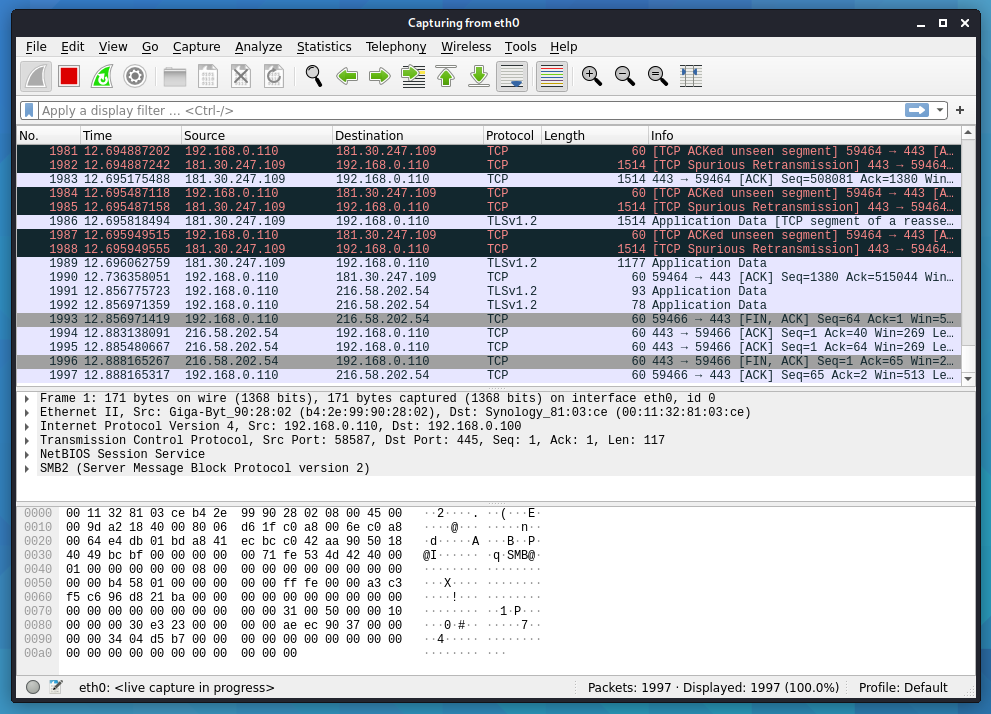
\includegraphics[width=10cm,height=7cm]{wireshark.png}
       \end{center}
       \caption{Interface del Wireshark}
    \end{figure}
 \end{center}
 
\subsubsection*{Ettercap}

\begin{center}
   \begin{figure}   
      \begin{center}
         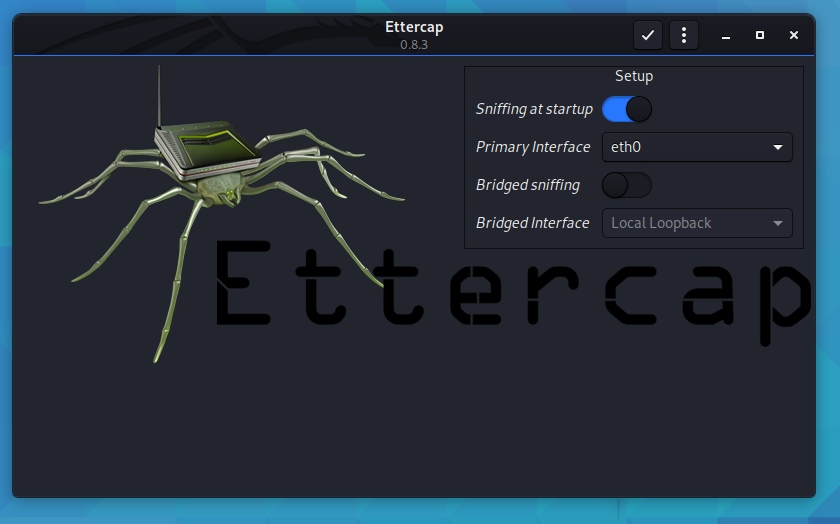
\includegraphics[width=10 cm,height=7cm]{ataque-2.png}
      \end{center}
      \caption{Ettercap}
   \end{figure}
\end{center}

Ettercap es un paquete completo gratuito y de código abierto para ataques basados 
en intermediarios. Ettercap se puede utilizar para análisis de protocolos de redes 
informáticas y auditorías de seguridad, con funciones de rastreo de conexiones en 
tiempo real y filtrado de contenido. Ettercap funciona configurando la interfaz de red 
del atacante en modo promiscuo y \emph{ARP} para envenenar las máquinas víctimas.



\subsection{Realización del ataque}

\begin{center}
    \begin{figure}   
       \begin{center}
          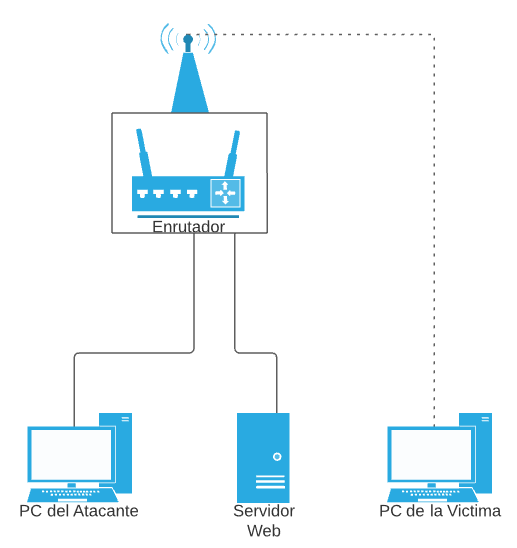
\includegraphics[width=9cm,height=9cm]{red.png}
       \end{center}
       \caption{Escenario montado}
    \end{figure}
 \end{center}

La idea principal de esta sección es demostrar que, encontrándose en una red interna
y con herramientas ya desarrolladas y libres, es posible realizar un ataque 
sin necesidad de conocer a fondo la implementación de la misma ni de tener mayores
privilegios.

El escenario consiste en crear una página web con un 
simple formulario donde se debe completar con usuario y contraseña, y un 
submit el cual envía esta información desde el cliente hasta el 
servidor web. El envío de este formulario contiene la información confidencial,
 por lo que en un escenario seguro ningún
intermediario podría obtener estos datos. Dado que este tráfico va a 
circular por HTTP, demostraremos como nos podemos hacer de las credenciales
ingresadas por el usuario.

\begin{center}
   \begin{figure}   
      \begin{center}
         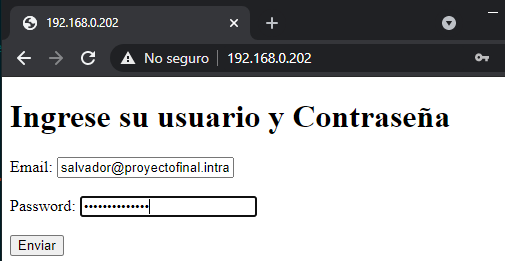
\includegraphics[width=10cm,height=6cm]{form.png}
      \end{center}
      \caption{Formulario montado}
   \end{figure}
\end{center}

Recordar que esto fue realizado en una red interna donde son todos equipos de nuestra propiedad.


\subsection{Preparando Ettercap para el ataque ARP Poisoning}

Lo primero que debemos hacer, en la lista de aplicaciones, es buscar el apartado 
\emph{Sniffing} y \emph{Spoofing}, ya que es allí donde encontraremos las herramientas necesarias
 para llevar a cabo este ataque. A continuación, abriremos Ettercap.

\begin{center}
    \begin{figure}   
       \begin{center}
          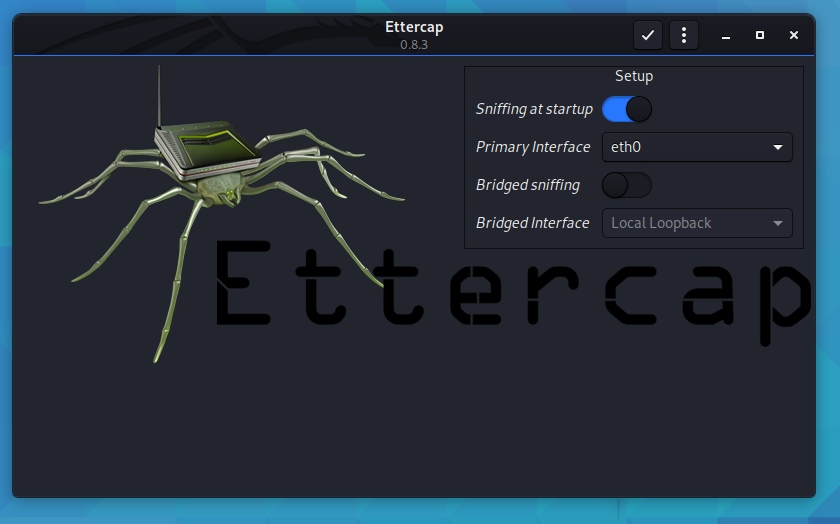
\includegraphics[width=9 cm,height=6cm]{ataque-2.png}
       \end{center}
       \caption{Ettercap}
    \end{figure}
 \end{center}

El siguiente paso es seleccionar la tarjeta de red con la que vamos a trabajar. Para 
ello, en el menú superior de Ettercap seleccionaremos Sniff $>$ Unified Sniffing y, 
cuando nos lo pregunte, seleccionaremos nuestra tarjeta de red (por ejemplo, en 
nuestro caso, eth0).

Luego se debe buscar todos los hosts conectados a nuestra red local. Para ello, 
seleccionaremos Hosts del menú de la parte superior y seleccionaremos la primera 
opción, Hosts List.

Allí deberían salirnos todos los hosts o dispositivos conectados a nuestra red. 
Sin embargo, en caso de que no salgan todos, podemos realizar una exploración 
completa de la red simplemente abriendo el menú Hosts y seleccionando la opción 
Scan for hosts. Tras unos segundos, la lista de antes se debería actualizar 
mostrando todos los dispositivos, con sus respectivas IPs y MACs, conectados 
a nuestra red.



\subsection{Nuestro Ettercap ya está listo. Ya podemos empezar con el ataque ARP Poisoning}

En caso de querer realizar un ataque dirigido contra un solo host, por ejemplo, 
suplantar la identidad de la puerta de enlace para monitorear las conexiones 
de la víctima, antes de empezar con el 
ataque debemos establecer los dos objetivos.

Para ello, debajo de la lista de hosts podemos ver tres botones, aunque nosotros 
prestaremos atención a los dos últimos:

    Target 1 – Seleccionamos la IP del dispositivo a monitorear, en este caso, 
    la computadora de la víctima, y pulsamos sobre dicho botón.

    Target 2 – Pulsamos la IP que queremos suplantar, en este caso, la de la 
    puerta de enlace y la del servidor web.

    \begin{center}
        \begin{figure}   
           \begin{center}
              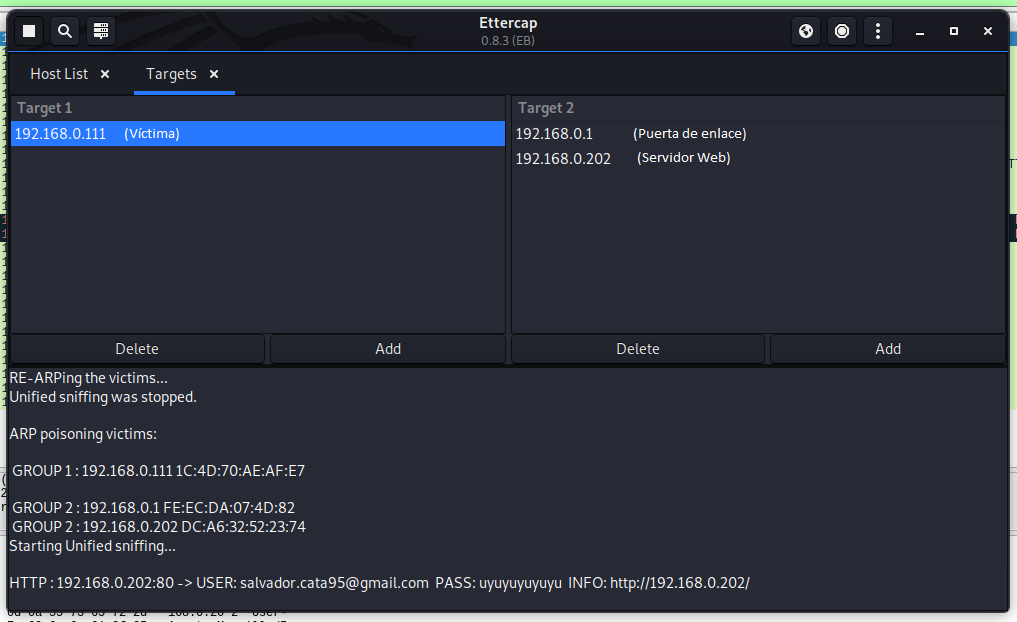
\includegraphics[width=17cm,height=9.5cm]{ataque-7-deta.png}
           \end{center}
           \caption{Ettercap}
        \end{figure}
     \end{center}

Todo listo. Ahora solo debemos elegir el menú MITM de la parte superior y, en él, 
escoger la opción ARP Poisoning. Nos aparecerá una pequeña ventana de configuración, 
en la cual debemos asegurarnos de marcar Sniff Remote Connections.
Pulsamos sobre Ok y el ataque dará lugar. Ahora ya podemos tener el control 
sobre el host que hayamos establecido como Target 1. Lo siguiente que debemos 
hacer es, ejecutar Wireshark para capturar todos los paquetes de 
red y analizarlos en busca de información interesante.

\begin{center}
   \begin{figure}   
      \begin{center}
         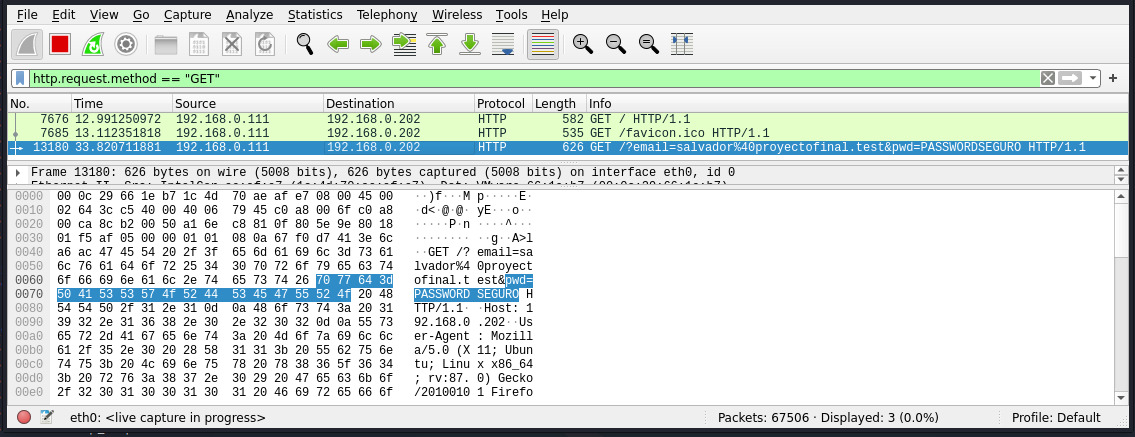
\includegraphics[width=17cm,height=7cm]{paquetes.png}
      \end{center}
      \caption{Paquetes capturados}
   \end{figure}
\end{center}

Como se puede ver, Wireshark nos permite filtrar el tráfico, y con el 
simple hecho de decirle que queremos mostrar los requerimientos GET
pudimos dar con el paquete que queríamos, en el request podemos ver
el usuario “salvador@proyectofinal.test” y la contraseña “PASSWORD SEGURO”


